\documentclass[11pt]{article}

\usepackage{amsmath,amssymb}
\usepackage[usenames,dvipsnames,svgnames,table]{xcolor}
\usepackage[colorlinks=true,citecolor=blue]{hyperref}
\usepackage{natbib}
\usepackage{graphicx}

\begin{document}

%%%%%%%%%
\title{SpeciesNetwork Tutorial \\
\large Inferring Species Networks from Multilocus Data}
\author{Chi Zhang \\
E-mail: zhangchi@ivpp.ac.cn}
\maketitle

%%%%%%%%%
\section*{Introduction}

This tutorial describes a full Bayesian framework for species network inference studying reticulate evolution. The statistical methodology is described in \citet{Zhang:2017gq}.
You will need the following software at your disposal:
\begin{itemize}
\item \textbf{BEAST} --- this package contains the BEAST program, BEAUti, and other utility programs. This tutorial is written for BEAST v2.4.7 or higher \citep[\url{http://beast2.org},][]{Bouckaert:2014iz}.
\item \textbf{Tracer} --- this program is used to explore the output of BEAST (and other Bayesian MCMC programs). It summarizes graphically and quantitively the distributions of continuous parameters and provides diagnostic information for the particular MCMC chain (\url{http://tree.bio.ed.ac.uk/software/tracer}).
\item \textbf{IcyTree} --- this is a web application for visualizing phylogenies, including phylogenetic networks \citep[\url{icytree.org};][]{Vaughan:2017fu}.
\end{itemize}

%%%%%%%%%
\section*{The Data}

The gene trees from six independent loci are simulated under the multispecies network coalescent \citep[MSNC;][]{Yu:2014dt} given the species network shown in figure \ref{fig_spnetwork}. Each gene tree has four tips per species. The sequence alignments are simulated under JC69 substitution model \citep{Jukes:1969wx} along the gene trees with strict molecular clock and no rate variation across loci. The sequence length is 200bp at each locus. The NEXUS file called \textbf{3s\_6loci.nex} is included with this tutorial.

\begin{figure}[h]
\center
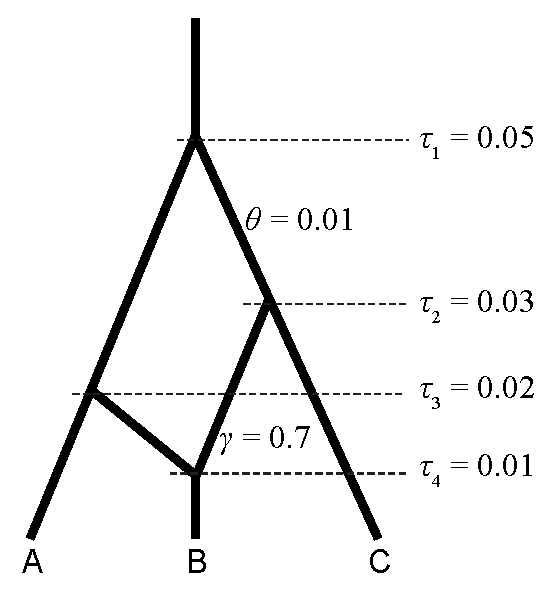
\includegraphics[width=0.5\textwidth]{figs/fig1_spnetwork}
\caption{Species network used to simulate the data}
\label{fig_spnetwork}
\end{figure}

The first step in the analysis will be to convert the NEXUS files into a BEAST XML input file. This is done using the program \textbf{BEAUti} included in the BEAST package. It is a user-friendly program for setting the evolutionary model and options for the MCMC analysis. The second step will be to actually run \textbf{BEAST} using the XML input file that contains the data, model and MCMC chain settings. The final step will be to explore the output of BEAST in order to diagnose problems and to summarize the results.

\section*{BEAUti}

\subsection*{Switching the template}

SpeciesNetwork uses a non-standard template to generate the XML, so the first thing to do is to change the template. Choose the \textbf{File / Template / SpeciesNetwork} item (fig. \ref{fig_template}). If you do not see this template in the menu, make sure the SpeciesNetwork plugin is installed correctly.
Keep in mind that when changing a template, BEAUti deletes all previously imported data and starts with a clean template. So, if you already loaded some data, a warning message will pop up indicating that this data will be lost if you switch templates.

\begin{figure}[h]
\center
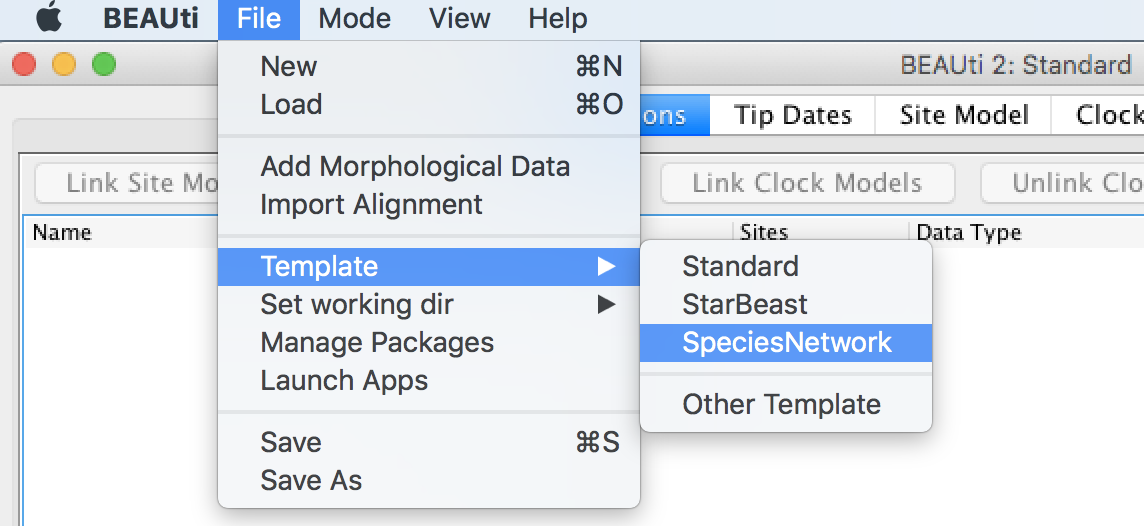
\includegraphics[width=0.7\textwidth]{figs/fig2_template}
\caption{Switching the template, then import the alignment}
\label{fig_template}
\end{figure}

\subsection*{Loading the NEXUS file}

To import the sequence alignment into BEAUti, use the \textbf{Import Alignment} option from the \textbf{File} menu (fig. \ref{fig_template}) and select \textbf{3s\_6loci.nex}. Once loaded, the six loci are displayed in the \textbf{Partitions} panel. You can double click any locus (partition) to show its detail.

\begin{figure}[h]
\center
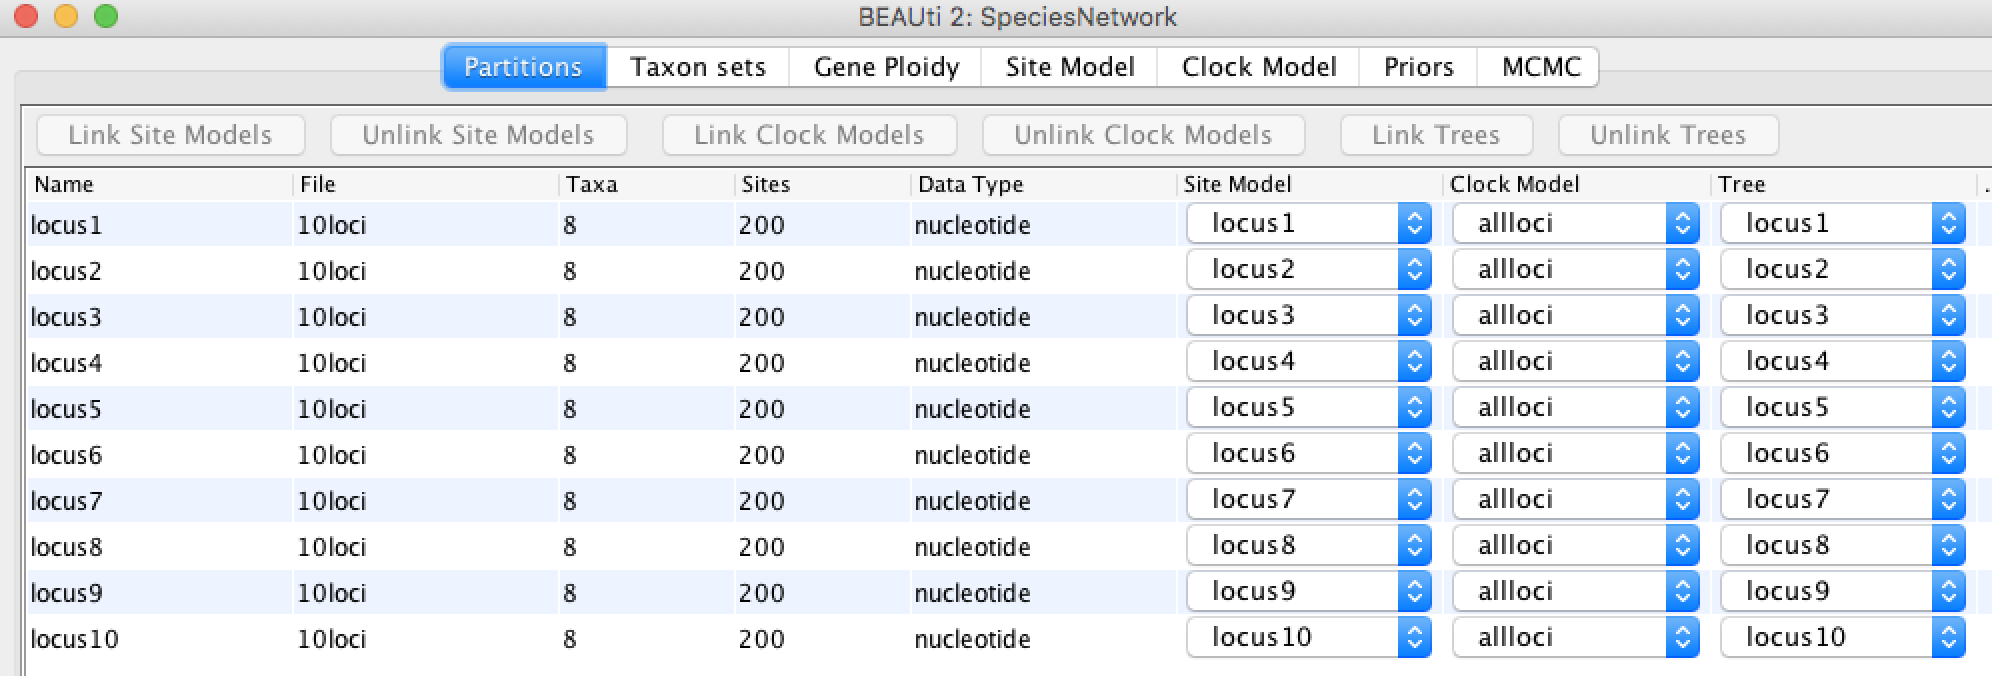
\includegraphics[width=1.0\textwidth]{figs/fig3_partition}
\caption{Partition panel after loading the alignment}
\label{fig_partition}
\end{figure}

For multilocus analyses, BEAST can link or unlink substitution, clock, and tree models across loci by clicking buttons at the top of the \textbf{Partitions} panel. The default is unlinking all models.
Since the species are contemporary and the implementation can not incorporate node calibrations (except for the origin), plus that the purpose here is not to explore evolutionary rate variation across gene tree lineages through relaxed clock models, we link the clock models for all loci and rename the label to \textbf{allloci} (fig. \ref{fig_partition}). The clock rate will later be fixed to 1.0 in the \textbf{Clock Model} panel. The evolutionary rate variation across different gene loci will be modeled using gene-rate multipliers and set in the \textbf{Site Model} panel (see below).
You should only unlink the tree models across loci that are actually genetically unlinked. For example, in most organisms all the mitochondrial genes are effectively linked due to a lack of recombination and they should be set up to use the same tree model.

\subsection*{Assigning taxa to species}
Each taxon should be assigned to a species, and this mapping is fixed during the analysis. Typically, the species name is already embedded inside the taxon name and should be easily extracted. If the default guess by BEAUti is not satisfactory, press the \textbf{Guess} button at the bottom and a dialog will show up where you can choose from several ways to try to detect the species names. Otherwise the names can be filled in manually (fig. \ref{fig_mapping}).

\begin{figure}[h]
\center
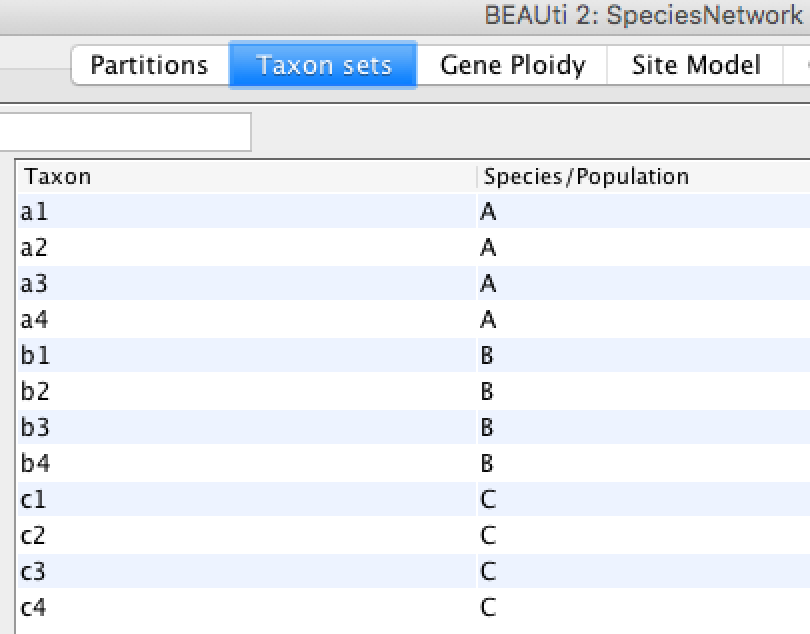
\includegraphics[width=0.6\textwidth]{figs/fig4_mapping}
\caption{Assigning taxa to species}
\label{fig_mapping}
\end{figure}

\subsection*{Setting gene ploidy}

Ploidy should be based on the mode of inheritance for each gene. By convention, nuclear genes in diploids are given a ploidy of 2.0. Because mitochondrial and Y chromosome genes are haploid even in otherwise diploid organisms, and also inherited only through the mother or the father respectively, their effective population size is only one quarter that of nuclear genes. Therefore if nuclear gene ploidy is set to 2.0, mitochondrial or Y chromosome gene ploidy should be set to 0.5. All genes in the simulation are assumed from nuclear loci and their ploidy should be left at the default value of 2.0 in the \textbf{Gene Ploidy} panel.

\subsection*{Setting up substitution and clock models}

The next thing to do is to set up the substitution and clock models.
Although the true substitution model in the simulation is JC69 which is the default in the \textbf{Site Model} panel, we select the \textbf{HKY} model \citep{Hasegawa:1985ww} that will fit better for real data. The frequencies are set to \textbf{empirical} so that only the $\kappa$ parameter is \textbf{estimated} (fig. \ref{fig_sitemodel}).
To account for evolutionary rate variation across loci with mean 1.0, tick \textbf{estimate} at \textbf{Substitution Rate} (fig. \ref{fig_sitemodel}) to use the gene-rate multipliers.

\begin{figure}[h]
\center
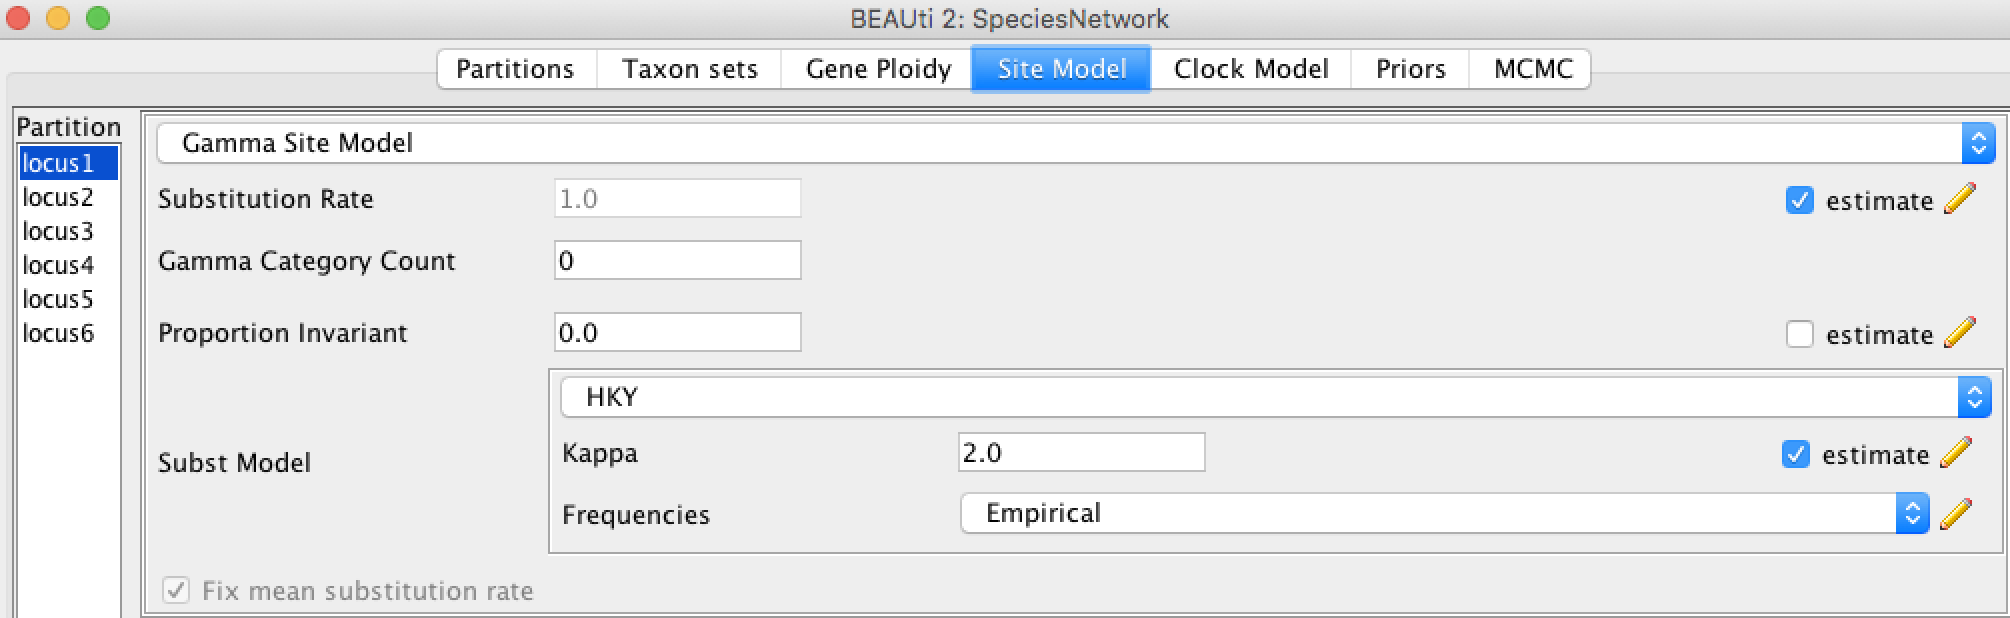
\includegraphics[width=1.0\textwidth]{figs/fig5_sitemodel}
\caption{Setting up substitution models}
\label{fig_sitemodel}
\end{figure}

Uncheck \textbf{estimate} in the \textbf{Clock Model} panel to fix the clock rate to 1.0 for all loci.
\begin{figure}[h]
\center
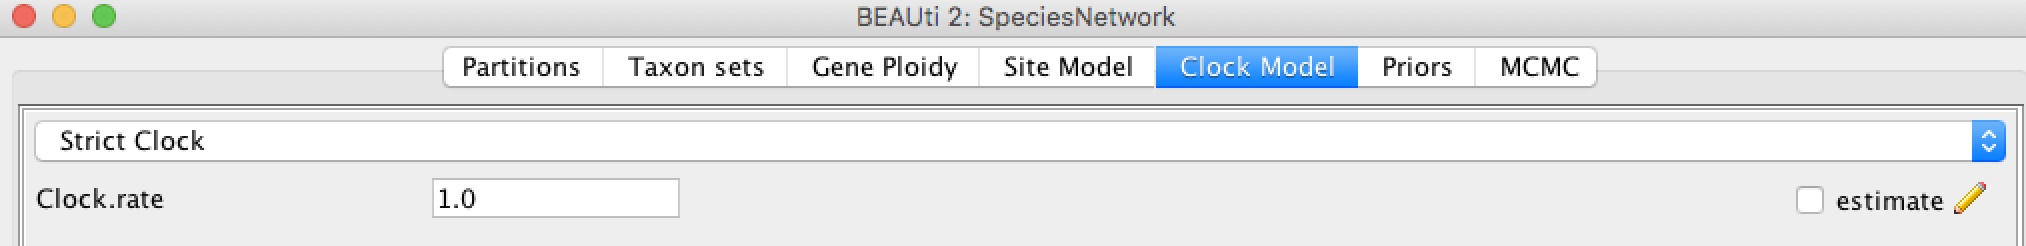
\includegraphics[width=1.0\textwidth]{figs/fig6_clockmodel}
\caption{Setting up clock models}
\label{fig_clockmodel}
\end{figure}

\subsection*{Changing the default priors}

The \textbf{Priors} panel allows priors for each parameter in the model to be specified. The default priors that BEAST sets for the parameters would allow the analysis to work. However, some of these are inappropriate for this analysis. Therefore change the priors as follows (fig. \ref{fig_priors}):

\begin{figure}[h]
\center
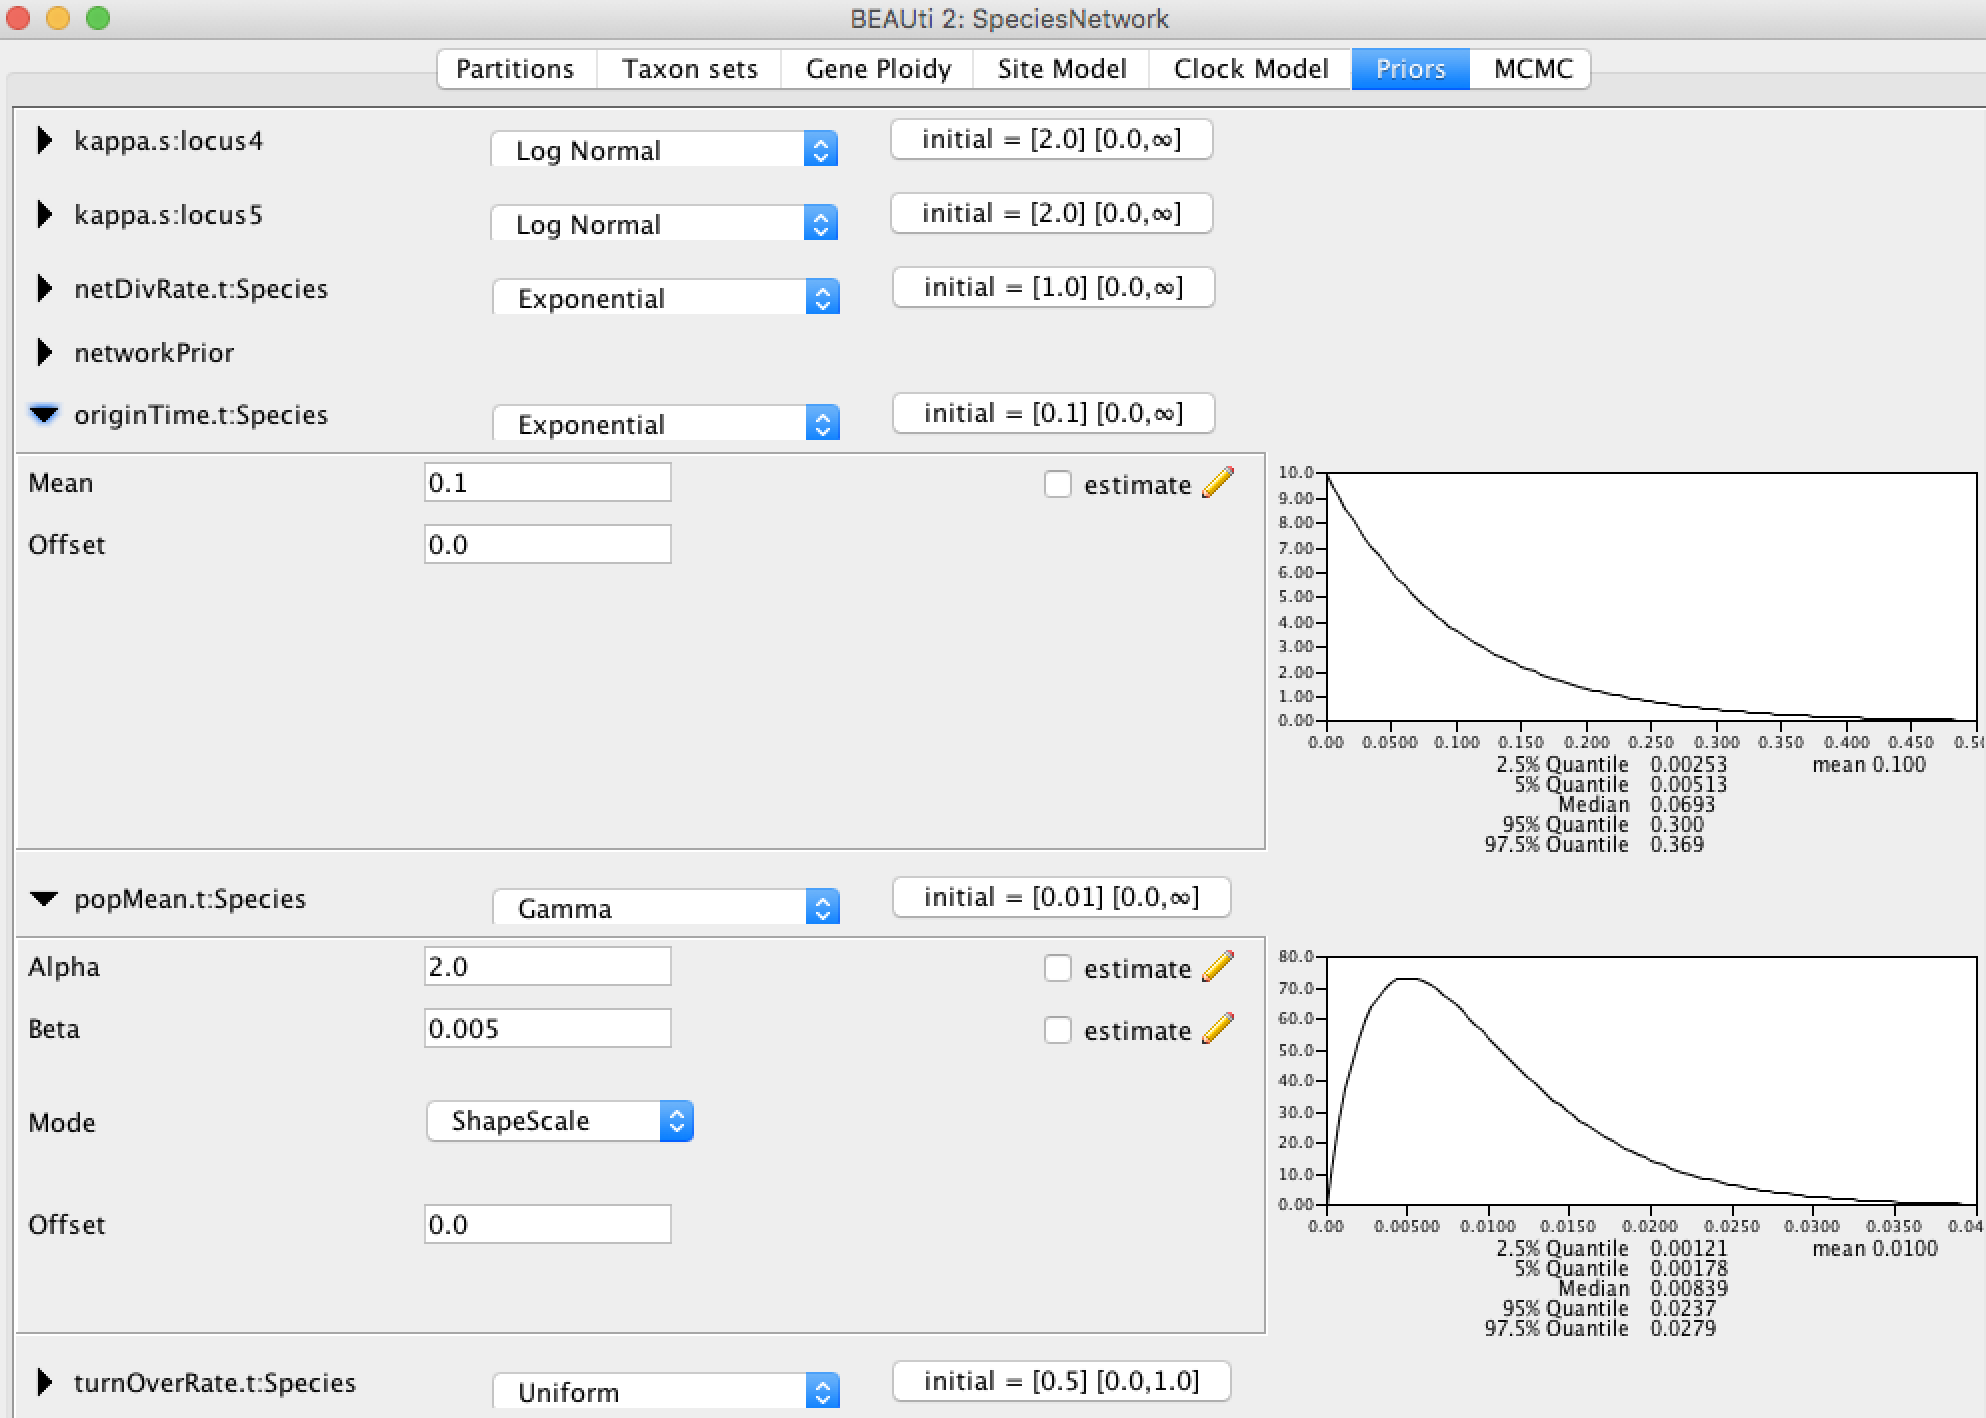
\includegraphics[width=1.0\textwidth]{figs/fig7_priors}
\caption{Changing priors}
\label{fig_priors}
\end{figure}

\textbf{netDivRate.t:Species}: Exponential with mean 10.0. This is for the parameter $\lambda-\nu$ (speciation rate minus hybridization rate). The other parameter \textbf{turnOverRate.t:Species} $=\nu/\lambda$ has the default prior $U(0,1)$.

\textbf{originTime.t:Species}: Exponential with mean 0.1. This is for the origin time of the species network. 

\textbf{popMean.t:Species}: Gamma with shape 2.0 and scale 0.005 (mean = 0.01). The population sizes of the species network are integrated out analytically using inverse-gamma(3, 2$\theta$) conjugate prior with mean $\theta$. This sets the prior for $\theta$.

\subsection*{Setting the MCMC options}

The \textbf{MCMC} tab provides settings for the MCMC chain. For this analysis, we set the \textbf{Chain Length} to \underline{20,000,000} (fig. \ref{fig_mcmc}). The appropriate length of the chain depends on the size of the dataset, the complexity of the model and the accuracy of the answer required, and should be adjusted accordingly. 
Increase \textbf{Log Every} under \textbf{screenlog} to \underline{10,000} to output less frequently to the screen, and decrease \textbf{Log Every} to \underline{2000} under \textbf{tracelog}, \textbf{specieslog}, and \textbf{treelog.t} so that \underline{20,000,000 / 2000 = 10,000} samples will be recorded in the log files (fig. \ref{fig_mcmc}). You can also change the \textbf{File Name} if you want.

\begin{figure}[h]
\center
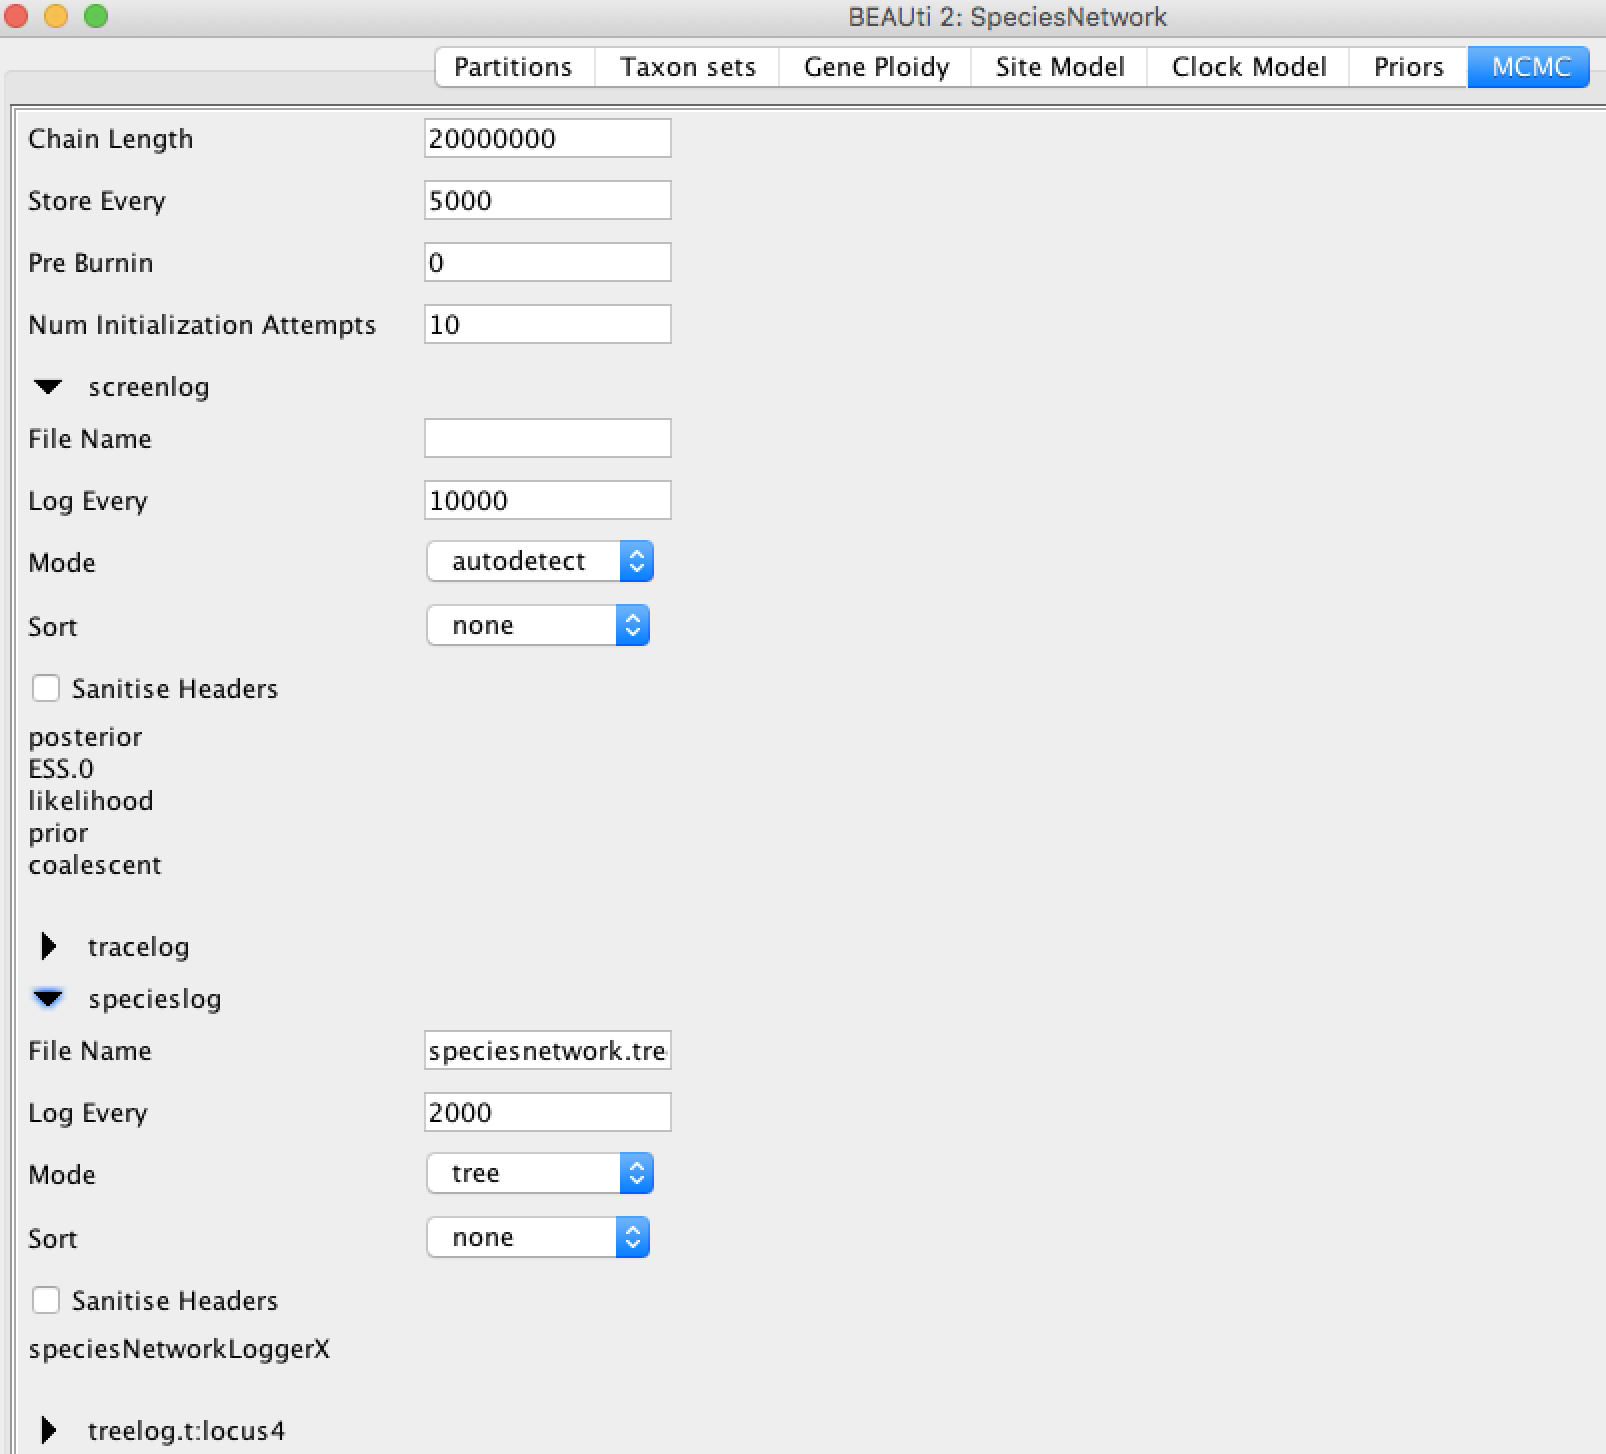
\includegraphics[width=0.9\textwidth]{figs/fig8_mcmc}
\caption{MCMC settings}
\label{fig_mcmc}
\end{figure}

\subsection*{Generating the BEAST XML input file}
We are now ready to create the BEAST XML file. To do this, either select the \textbf{File/Save} or \textbf{File/Save As} option from the \textbf{File} menu. Save the file with an appropriate name (i.e., \textbf{3s\_6loci.xml}). We are now ready to run the file through BEAST.

\section*{BEAST}

Now run BEAST. Provide your newly created XML file as input by clicking \textbf{Choose File}, and then click \textbf{Run} (Fig.~\ref{fig_beast}).

\begin{figure}[h]
\center
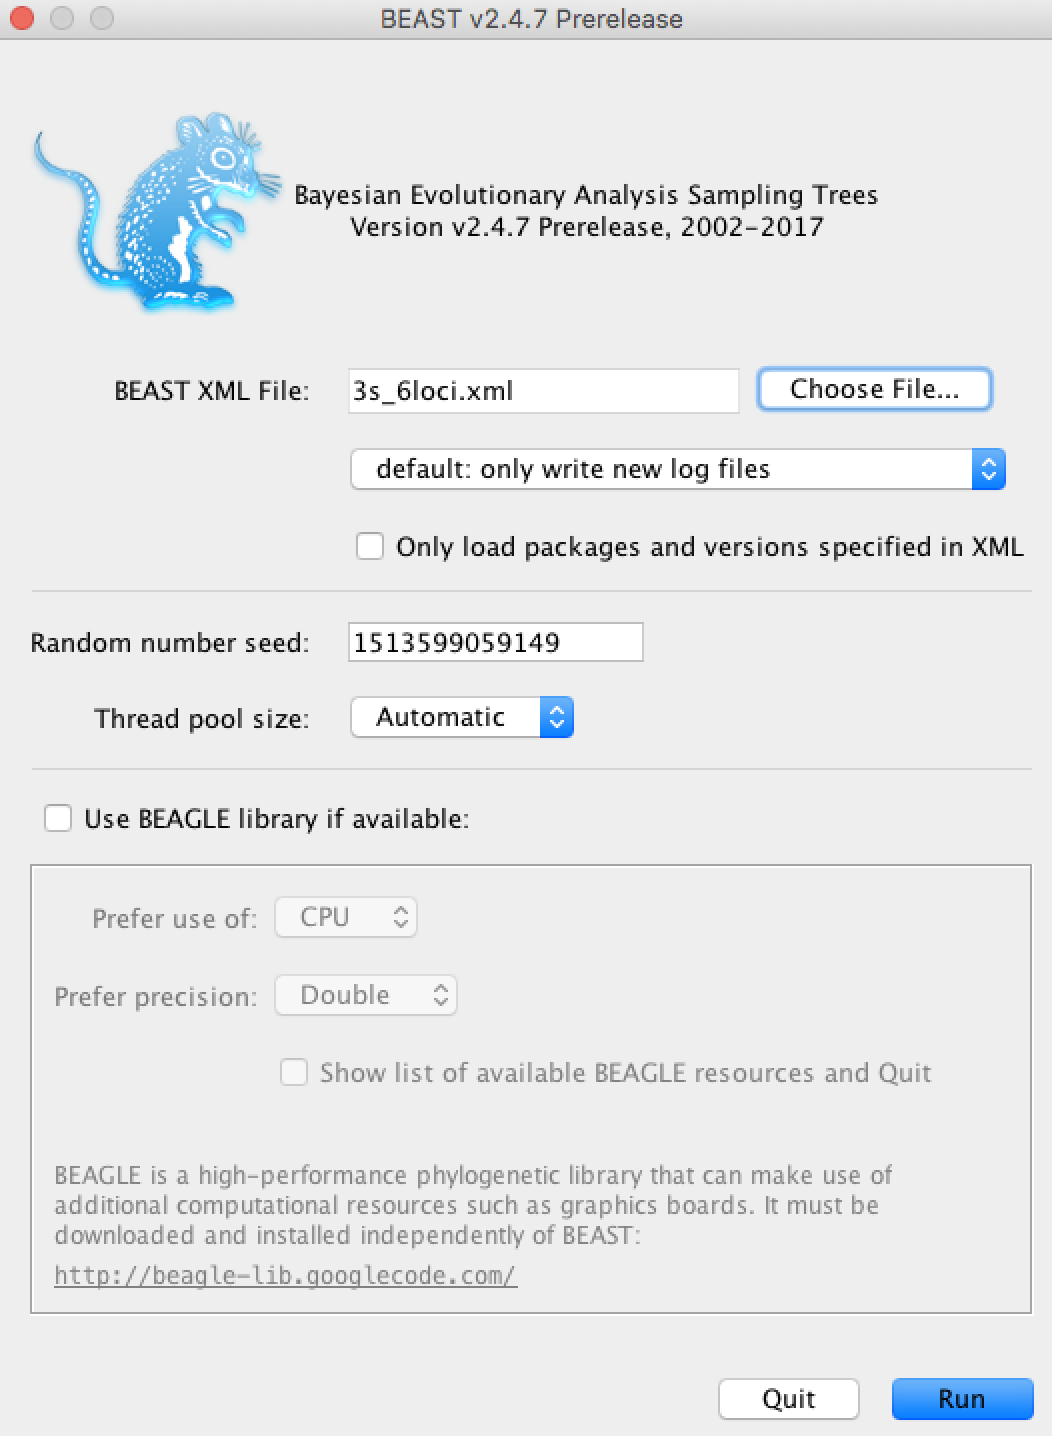
\includegraphics[width=0.6\textwidth]{figs/fig9_beast}
\caption{Launching BEAST}
\label{fig_beast}
\end{figure}

BEAST will then run until the specified chain length is reached and has finished reporting information on the screen. The actual result files are saved to the disk in the same location as your input file. The output to the screen will look something like this: 

{\tiny   
\begin{verbatim}
                        BEAST v2.4.7, 2002-2017
             Bayesian Evolutionary Analysis Sampling Trees
                       Designed and developed by
 Remco Bouckaert, Alexei J. Drummond, Andrew Rambaut & Marc A. Suchard
                                    
                     Department of Computer Science
                         University of Auckland
                        remco@cs.auckland.ac.nz
                        alexei@cs.auckland.ac.nz
                                    
                   Institute of Evolutionary Biology
                        University of Edinburgh
                           a.rambaut@ed.ac.uk
                                    
                    David Geffen School of Medicine
                 University of California, Los Angeles
                           msuchard@ucla.edu
                                    
                      Downloads, Help & Resources:
                           http://beast2.org/
                                    
  Source code distributed under the GNU Lesser General Public License:
                   http://github.com/CompEvol/beast2
                                    
                           BEAST developers:
   Alex Alekseyenko, Trevor Bedford, Erik Bloomquist, Joseph Heled, 
 Sebastian Hoehna, Denise Kuehnert, Philippe Lemey, Wai Lok Sibon Li, 
Gerton Lunter, Sidney Markowitz, Vladimir Minin, Michael Defoin Platel, 
                 Oliver Pybus, Chieh-Hsi Wu, Walter Xie
                                    
                               Thanks to:
          Roald Forsberg, Beth Shapiro and Korbinian Strimmer

Random number seed: 1513599534398

... ...

       19980000     -3755.2854       291.9        -3924.4938        -5.8601       175.0685 1m11s/Msamples
       19990000     -3748.1806       291.2        -3919.6018        -5.0581       176.4793 1m11s/Msamples
       20000000     -3739.4383       290.2        -3920.0553        -4.7404       185.3575 1m11s/Msamples

Operator                                                                   Tuning #accept #reject Pr(m) Pr(acc|m)
speciesnetwork.operators.RebuildEmbedding(scaleAndEmbed.t:locus1)               -   10176   80612 0.0022 0.1121 
speciesnetwork.operators.RebuildEmbedding(scaleRootAndEmbed.t:locus1)           -   18115   72451 0.0022 0.2000 
speciesnetwork.operators.RebuildEmbedding(uniformAndEmbed.t:locus1)             -  387402  517058 0.0217 0.4283 
speciesnetwork.operators.RebuildEmbedding(subSlideAndEmbed.t:locus1)            -    2355  450766 0.0108 0.0052 
speciesnetwork.operators.RebuildEmbedding(narrowAndEmbed.t:locus1)              -   86536  366085 0.0108 0.1912 
speciesnetwork.operators.RebuildEmbedding(wideAndEmbed.t:locus1)                -    2134  148900 0.0036 0.0141 
speciesnetwork.operators.RebuildEmbedding(WilsonBaldingAndEmbed.t:locus1)       -    1610  148889 0.0036 0.0107 
speciesnetwork.operators.RebuildEmbedding(scaleAndEmbed.t:locus3)               -    9335   80955 0.0022 0.1034 
speciesnetwork.operators.RebuildEmbedding(scaleRootAndEmbed.t:locus3)           -   20730   69727 0.0022 0.2292 
speciesnetwork.operators.RebuildEmbedding(uniformAndEmbed.t:locus3)             -  370569  534347 0.0217 0.4095 
speciesnetwork.operators.RebuildEmbedding(subSlideAndEmbed.t:locus3)            -    2302  450354 0.0108 0.0051 
speciesnetwork.operators.RebuildEmbedding(narrowAndEmbed.t:locus3)              -   55750  397314 0.0108 0.1231 
speciesnetwork.operators.RebuildEmbedding(wideAndEmbed.t:locus3)                -    1523  149702 0.0036 0.0101 
speciesnetwork.operators.RebuildEmbedding(WilsonBaldingAndEmbed.t:locus3)       -    1302  149760 0.0036 0.0086 
speciesnetwork.operators.RebuildEmbedding(scaleAndEmbed.t:locus6)               -   11934   78415 0.0022 0.1321 
speciesnetwork.operators.RebuildEmbedding(scaleRootAndEmbed.t:locus6)           -   20158   70611 0.0022 0.2221 
speciesnetwork.operators.RebuildEmbedding(uniformAndEmbed.t:locus6)             -  314749  592227 0.0217 0.3470 
speciesnetwork.operators.RebuildEmbedding(subSlideAndEmbed.t:locus6)            -    2290  449479 0.0108 0.0051 
speciesnetwork.operators.RebuildEmbedding(narrowAndEmbed.t:locus6)              -   30934  421088 0.0108 0.0684 
speciesnetwork.operators.RebuildEmbedding(wideAndEmbed.t:locus6)                -     554  150583 0.0036 0.0037 
speciesnetwork.operators.RebuildEmbedding(WilsonBaldingAndEmbed.t:locus6)       -     623  149598 0.0036 0.0041 
speciesnetwork.operators.RebuildEmbedding(scaleAndEmbed.t:locus2)               -   15785   74034 0.0022 0.1757 
speciesnetwork.operators.RebuildEmbedding(scaleRootAndEmbed.t:locus2)           -   22237   68347 0.0022 0.2455 
speciesnetwork.operators.RebuildEmbedding(uniformAndEmbed.t:locus2)             -  389666  515453 0.0217 0.4305 
speciesnetwork.operators.RebuildEmbedding(subSlideAndEmbed.t:locus2)            -    2300  450835 0.0108 0.0051 
speciesnetwork.operators.RebuildEmbedding(narrowAndEmbed.t:locus2)              -   77472  375767 0.0108 0.1709 
speciesnetwork.operators.RebuildEmbedding(wideAndEmbed.t:locus2)                -    2474  149238 0.0036 0.0163 
speciesnetwork.operators.RebuildEmbedding(WilsonBaldingAndEmbed.t:locus2)       -    2070  148970 0.0036 0.0137 
speciesnetwork.operators.RebuildEmbedding(scaleAndEmbed.t:locus5)               -   19502   71012 0.0022 0.2155 
speciesnetwork.operators.RebuildEmbedding(scaleRootAndEmbed.t:locus5)           -   18816   71609 0.0022 0.2081 
speciesnetwork.operators.RebuildEmbedding(uniformAndEmbed.t:locus5)             -  391190  516126 0.0217 0.4312 
speciesnetwork.operators.RebuildEmbedding(subSlideAndEmbed.t:locus5)            -    2329  450527 0.0108 0.0051 
speciesnetwork.operators.RebuildEmbedding(narrowAndEmbed.t:locus5)              -  146313  306000 0.0108 0.3235 
speciesnetwork.operators.RebuildEmbedding(wideAndEmbed.t:locus5)                -    3046  147868 0.0036 0.0202 
speciesnetwork.operators.RebuildEmbedding(WilsonBaldingAndEmbed.t:locus5)       -    2213  148708 0.0036 0.0147 
speciesnetwork.operators.RebuildEmbedding(scaleAndEmbed.t:locus4)               -   10385   80421 0.0022 0.1144 
speciesnetwork.operators.RebuildEmbedding(scaleRootAndEmbed.t:locus4)           -   19474   71037 0.0022 0.2152 
speciesnetwork.operators.RebuildEmbedding(uniformAndEmbed.t:locus4)             -  312247  592369 0.0217 0.3452 
speciesnetwork.operators.RebuildEmbedding(subSlideAndEmbed.t:locus4)            -    2355  450564 0.0108 0.0052 
speciesnetwork.operators.RebuildEmbedding(narrowAndEmbed.t:locus4)              -   68066  385324 0.0108 0.1501 
speciesnetwork.operators.RebuildEmbedding(wideAndEmbed.t:locus4)                -    1361  148858 0.0036 0.0091 
speciesnetwork.operators.RebuildEmbedding(WilsonBaldingAndEmbed.t:locus4)       -    1068  149890 0.0036 0.0071 
ScaleOperator(KappaScaler.s:locus1)                                        0.3251    9544   20727 0.0007 0.3153 
ScaleOperator(KappaScaler.s:locus2)                                        0.3049    8978   21083 0.0007 0.2987 
ScaleOperator(KappaScaler.s:locus3)                                        0.3219    8808   21598 0.0007 0.2897 
ScaleOperator(KappaScaler.s:locus4)                                        0.3217    9010   20999 0.0007 0.3002 
ScaleOperator(KappaScaler.s:locus5)                                        0.2738    9076   21028 0.0007 0.3015 
ScaleOperator(KappaScaler.s:locus6)                                        0.2992    9180   21042 0.0007 0.3038 
DeltaExchangeOperator(FixMeanMutationRatesOperator)                        0.6532   11826   48614 0.0014 0.1957 
ScaleOperator(popMeanScale.t:Species)                                      0.3051    9604   22933 0.0036 0.2952 
ScaleOperator(netDivRateScale.t:Species)                                   0.1444   17706   47785 0.0072 0.2704 
ScaleOperator(turnOverRateScale.t:Species)                                 0.0697   10361   55010 0.0072 0.1585 
speciesnetwork.operators.GammaProbUniform(gammaProbUniform.t:Species)           -   31549  164264 0.0217 0.1611 
speciesnetwork.operators.GammaProbRndWalk(gammaProbRndWalk.t:Species)           -   50895  143971 0.0217 0.2612 
speciesnetwork.operators.NetworkMultiplier(networkMultiplier.t:Species)         -   94308  100953 0.0217 0.4830 
speciesnetwork.operators.OriginMultiplier(originMultiplier.t:Species)      1.0000   29362    3080 0.0036 0.9051 
speciesnetwork.operators.RebuildEmbedding(nodeUniformAndEmbed.t:Species)        -   77611  574779 0.0723 0.1190 
speciesnetwork.operators.RebuildEmbedding(nodeSliderAndEmbed.t:Species)         -  444951  206324 0.0723 0.6832 
speciesnetwork.operators.RebuildEmbedding(relocateBranchAndEmbed.t:Species)     -  101644 2505081 0.2890 0.0390 
speciesnetwork.operators.RebuildEmbedding(addReticulationAndEmbed.t:Species)    -    9886  641888 0.0723 0.0152 
speciesnetwork.operators.RebuildEmbedding(deleteReticulationAndEmbed.t:Species) -    9884  641331 0.0723 0.0152 

     Tuning: The value of the operator's tuning parameter, or '-' if the operator can't be optimized.
    #accept: The total number of times a proposal by this operator has been accepted.
    #reject: The total number of times a proposal by this operator has been rejected.
      Pr(m): The probability this operator is chosen in a step of the MCMC (i.e. the normalized weight).
  Pr(acc|m): The acceptance probability (#accept as a fraction of the total proposals for this operator).

Total calculation time: 1439.539 seconds
End likelihood: -3739.4383147683425
\end{verbatim}}

It is strongly recommended to run multiple independent runs to confirm the results are consistent across runs. Then the log files can be combined using \textbf{LogCombiner} included in the BEAST package.

\section*{Analyzing the results}

\subsection*{Tracer}

Run the program called \textbf{Tracer} to analyze the output of BEAST. When the main window has opened, choose \textbf{Import Trace File} from the \textbf{File} menu and select the file that BEAST has created called \textbf{speciesnetwork.log}. Change the \textbf{Burn-In} to \underline{5,000,000} on the top-left so that the first 25\% samples are discarded.
On the left-hand side is a list of the different quantities that BEAST has logged. Selecting one item from this list brings up the trace under the \textbf{Trace} tab and the statistics for this trace under the \textbf{Estimates} tab on the right-hand side.

For example, select \textbf{popMean.t:Species} to display the estimate of mean population size (fig. \ref{fig_tracer1}), and select the six \textbf{mutationRate.s} items (hold \texttt{shift} key while selecting) to display the estimates of the gene-rate multipliers. If you switch the tab at the top of the right-hand side to {\bf Marginal Prob Distribution} then you will get a plot of the marginal posterior densities of the estimates overlaid (fig. \ref{fig_tracer2}).
Remember that MCMC is a stochastic algorithm so the actual numbers will not be exactly the same.

\subsection*{Viewing the species networks}

To summarize the posterior samples of species networks, we need to prepare another XML file specifying the input and output file names, and the burn-in (\underline{2501} out of 10,000 in this case). Save the following content to \textbf{3s\_6loci\_sum.xml} and put it to the same folder as the log files.

{\tiny
\begin{verbatim}
<?xml version='1.0' encoding='UTF-8'?>
<beast namespace="beast.core:beast.app" version="2.4">
    <run id="network.summary" spec="speciesnetwork.tools.SummarizePosterior"
         inputFileName="speciesnetwork.trees" outputFileName="speciesnetwork.sum.trees" burnin="2501"/>
</beast>
\end{verbatim}}

\begin{figure}[h]
\center
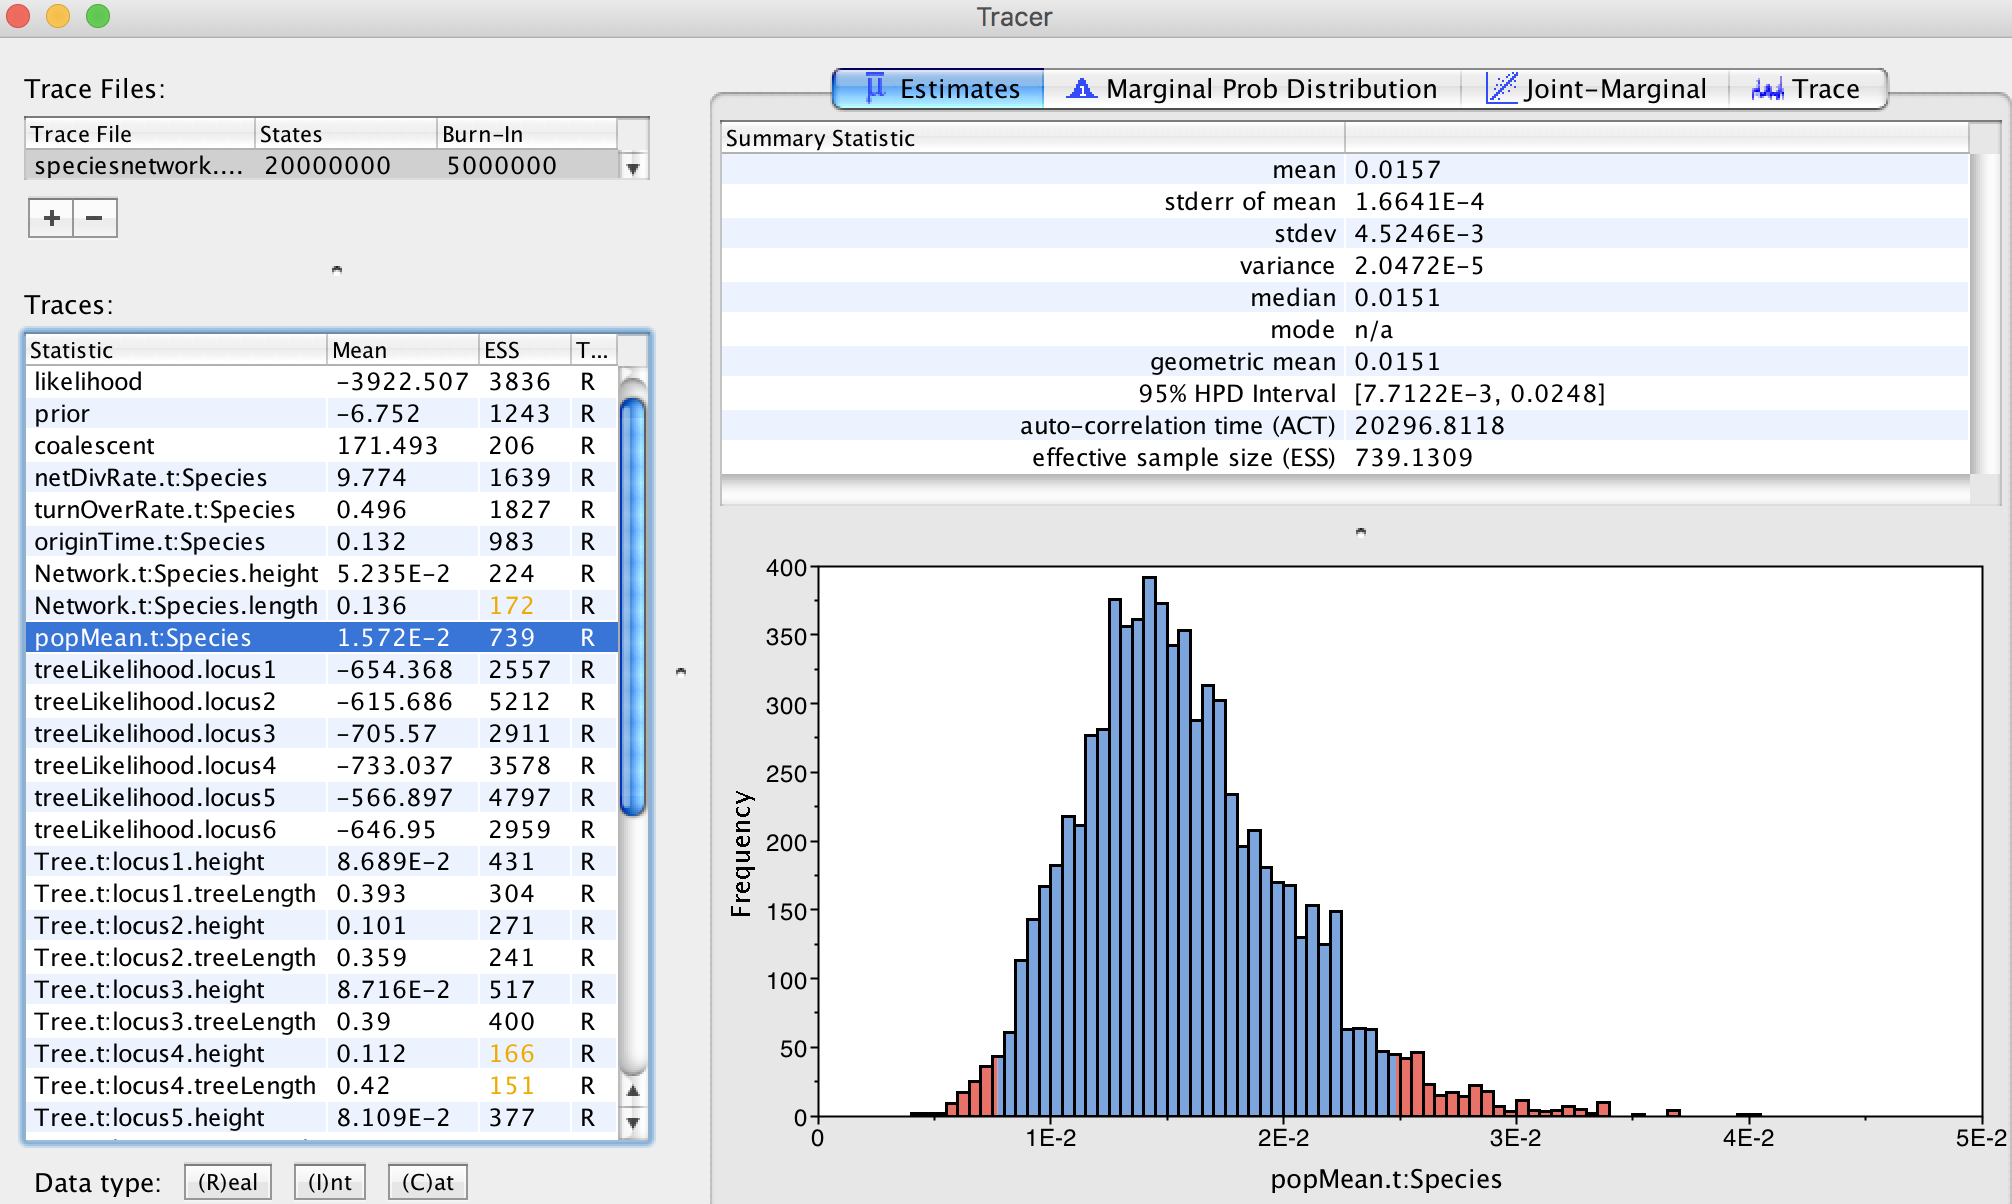
\includegraphics[width=1.0\textwidth]{figs/fig10_tracer1}
\caption{Tracer showing the estimate of mean population size}
\label{fig_tracer1}
\end{figure}

\begin{figure}[h]
\center
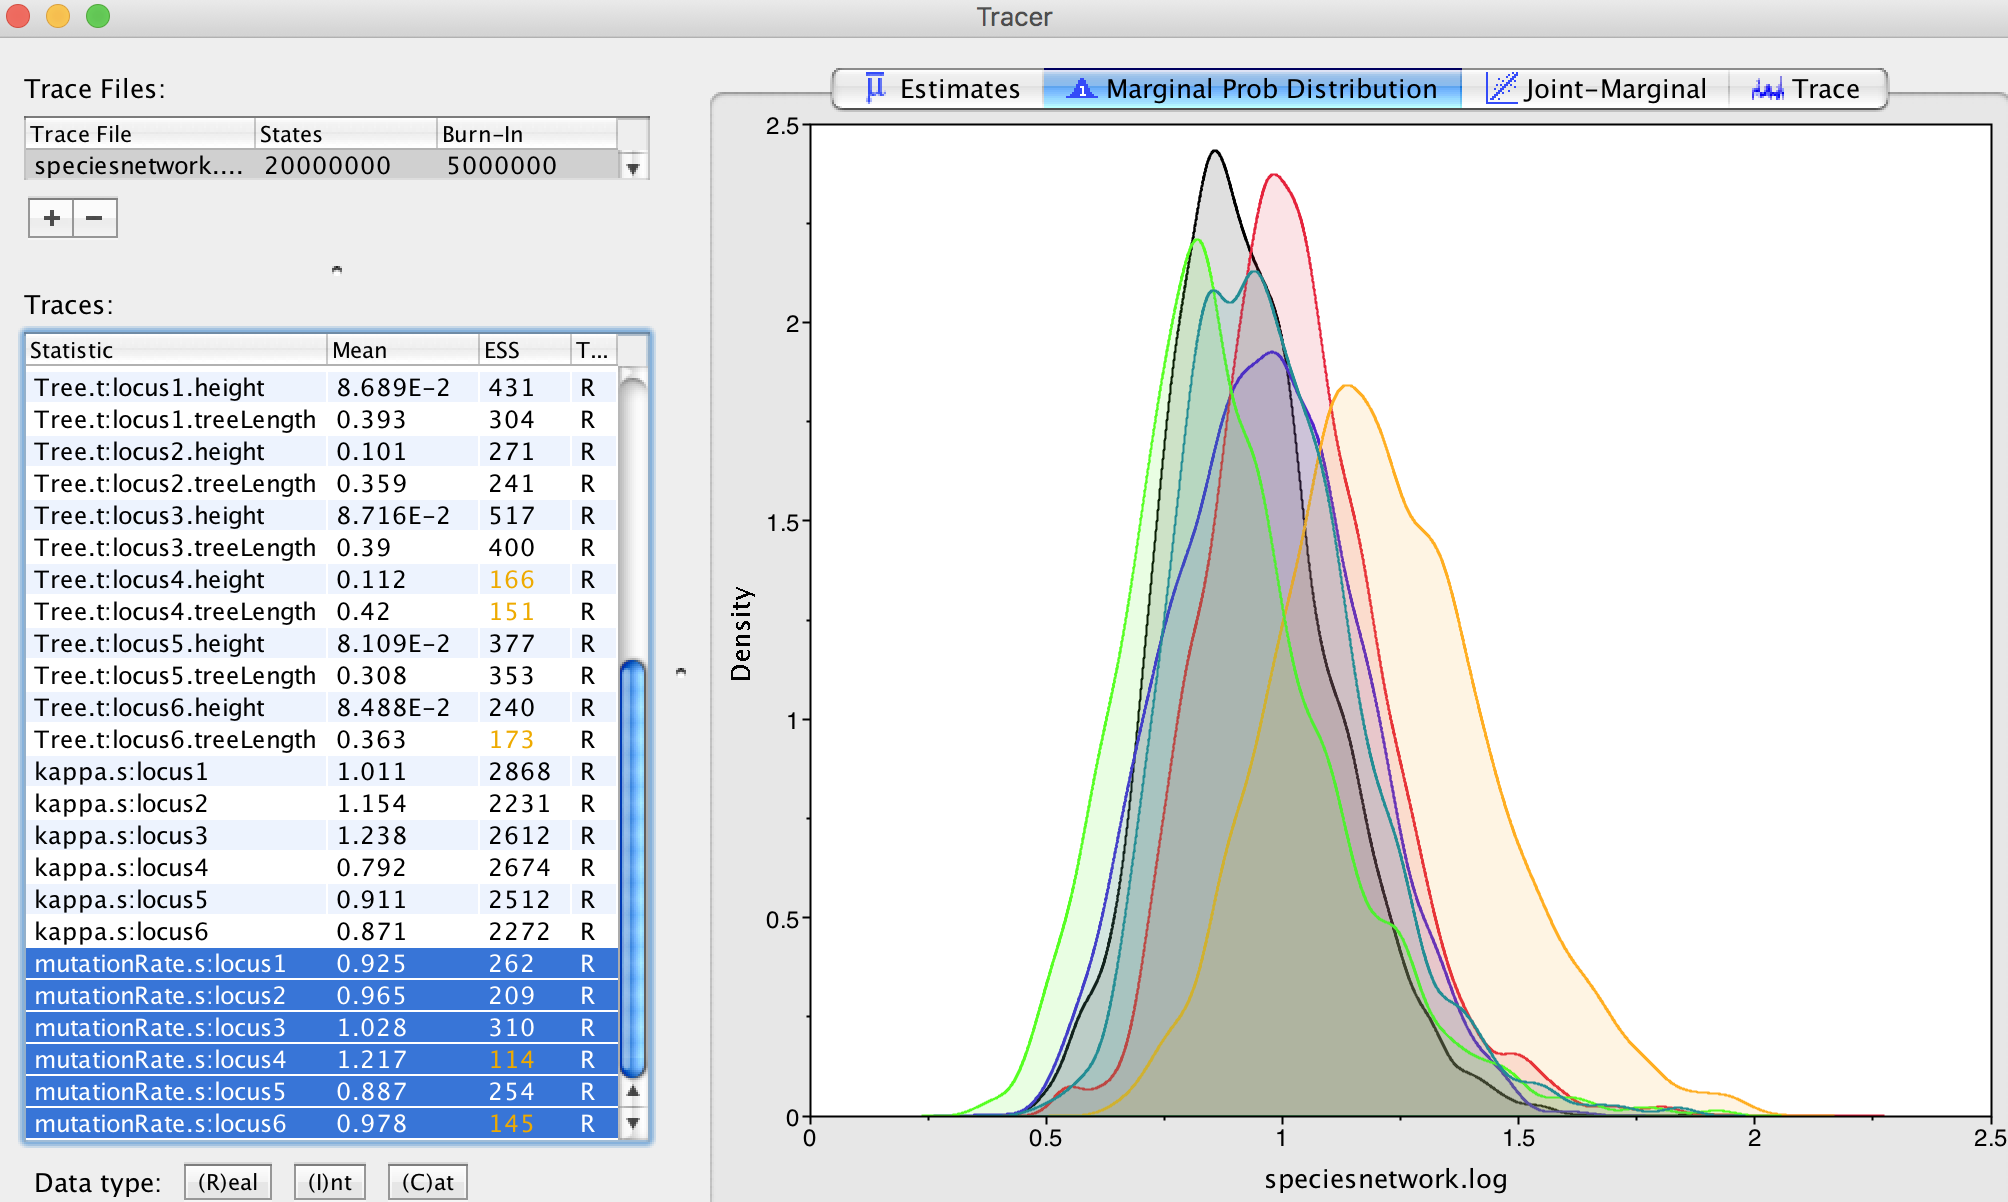
\includegraphics[width=1.0\textwidth]{figs/fig11_tracer2}
\caption{Tracer showing the marginal prob. of gene-rate multipliers}
\label{fig_tracer2}
\end{figure}
\clearpage

\noindent Then run BEAST as you did for the standard analysis above but with 3s\_6loci\_sum.xml as input. The summary networks will be saved to \textbf{speciesnetwork.sum.trees}. It contains unique network topologies in descending order of their posterior probabilities. For each unique topology, the summaries of node height and inheritance probability (if apply) are annotated for each node. 
Open \textbf{IcyTree} by entering the URL \url{icytree.org} to your browser. Then you can either drag and drop, or select \textbf{File / Load from file} to load the summary species networks in \textbf{speciesnetwork.sum.trees}. Select \textbf{Style / Internal node text / topologySupport} to display the posterior probability at the root for each network.

\begin{figure}[h]
\center
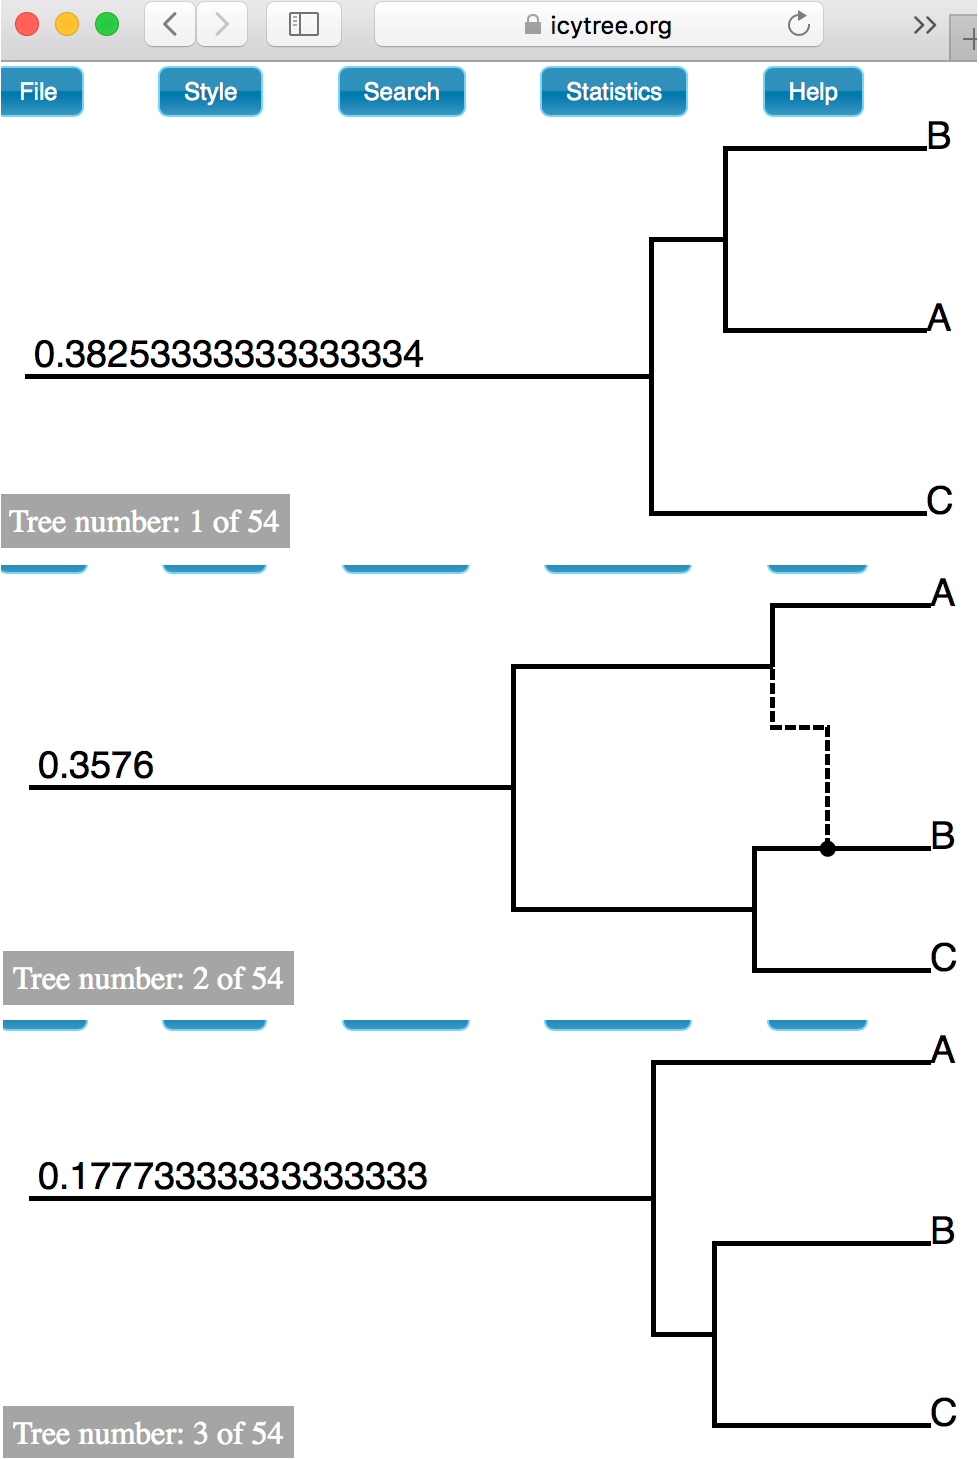
\includegraphics[width=0.6\textwidth]{figs/fig12_networks}
\caption{IcyTree showing the species networks}
\label{fig_networks}
\end{figure}

Figure \ref{fig_networks} shows the three species networks in the 95\% posterior credible set. The true species network with one hybridization has probability 0.36. The estimate of inheritance probability $\gamma$ is 0.51 (0.20, 0.78) while the true value is 0.3. This can be viewed in \textbf{Child attribs} by moving the cursor to the reticulation branch.

\bigskip
\noindent \href{http://creativecommons.org/licenses/by/4.0/}{
\includegraphics[scale=0.7]{figs/fig_ccby.pdf}} This tutorial is licensed under a \href{http://creativecommons.org/licenses/by/4.0/}{Creative Commons Attribution 4.0 International License}. 

%%%%%%%%%  REFERENCE    %%%%%%%%%%%%%%%
\bibliographystyle{mbe}
\bibliography{refs}

\end{document}
